\documentclass[11pt]{article}
\usepackage[hmargin=1in,vmargin=1in]{geometry}
\usepackage{xcolor}
\usepackage{amsmath,amssymb,amsfonts,url,sectsty,framed,tcolorbox,framed}
\newcommand{\pf}{{\bf Proof: }}
\newtheorem{theorem}{Theorem}
\newtheorem{lemma}{Lemma}
\newtheorem{proposition}{Proposition}
\newtheorem{definition}{Definition}
\newtheorem{remark}{Remark}
\newcommand{\qed}{\hfill \rule{2mm}{2mm}}
\newtheorem{example}{Example}
\usepackage{tikz}
\usepackage{bm}

\begin{document}
%%%%%%%%%%%%%%%%%%%%%%%%%%%%%%%%%%%%%%%%%%%%%%%%%%%%%%%%%%%%%%%%%%%%%
\noindent
\rule{\textwidth}{1pt}
\begin{center}
{\bf [CS304] Introduction to Cryptography and Network Security}
\end{center}
Course Instructor: Dr. Dibyendu Roy \hfill Winter 2023-2024\\
Scribed by: Raghav Agiwal (202151124) \hfill Lecture (Week 10)
\\
\rule{\textwidth}{1pt}
%%%%%%%%%%%%%%%%%%%%%%%%%%%%%%%%%%%%%%%%%%%%%%%s%%%%%%%%%%%%
%write here


\section{Chinese Remainder Theorem}

The Chinese Remainder Theorem (CRT) is a mathematical principle used to solve systems of congruences. Given a system of equations in the form:

\[
\begin{aligned}
x &\equiv a_1 \pmod{m_1} \\
x &\equiv a_2 \pmod{m_2} \\
&\vdots \\
x &\equiv a_r \pmod{m_r}
\end{aligned}
\]

where $m_1, m_2, \ldots, m_r$ are pairwise coprime integers, CRT guarantees the existence of a unique solution modulo $M = m_1 \cdot m_2 \cdot \ldots \cdot m_r$.

To solve such a system, we introduce the concept of $\delta_j$ for each $1 \leq j \leq r$:

\[
\delta_j =
\begin{cases}
1, & \text{mod } m_j \\
0, & \text{mod } m_i, \text{ if } i \neq j
\end{cases}
\]

Expressing the solution $x$ as a summation involving $a_j$ and $\delta_j$, we get:

\[
x = \sum_{j=1}^{r} a_j \cdot \delta_j
\]

By expanding $x$, we find:

\[
x = \delta_1 \cdot a_1 + \delta_2 \cdot a_2 + \ldots + \delta_r \cdot a_r \quad (\text{Eq. 1})
\]

For each equation $x \equiv a_j \pmod{m_j}$, taking modulus $m_j$ of $x$ leads to:

\[
x \equiv (\delta_1 \cdot a_1 + \delta_2 \cdot a_2 + \ldots + \delta_r \cdot a_r) \pmod{m_j}
\]

Since $\delta_i$ is 0 for $i \neq j$ and 1 for $j$, we obtain $x \equiv a_j \pmod{m_j}$, proving that $x$ is a solution.

To compute $\delta_j$ for each $j$, we determine $M = m_1 \cdot m_2 \cdot \ldots \cdot m_r$ and find the multiplicative inverse $b_j$ of $M \pmod{m_j}$. Then, $\delta_j$ is given by:

\[
\delta_j = \frac{M}{m_j} \cdot b_j
\]

CRT ensures uniqueness by demonstrating that any other solution $x'$ is congruent to $x \pmod{M}$, thus proving the uniqueness of the solution.

This theorem is a fundamental concept in number theory and has applications in various areas of mathematics and computer science.


\subsection{Explanation of the Chinese Remainder Theorem}

The Chinese Remainder Theorem (CRT) offers a method to solve a system of congruences, providing a unique solution under certain conditions.

Suppose we have a system of congruences:

\[
\begin{aligned}
x &\equiv a_1 \pmod{m_1} \\
x &\equiv a_2 \pmod{m_2} \\
&\vdots \\
x &\equiv a_r \pmod{m_r}
\end{aligned}
\]

where $m_1, m_2, \ldots, m_r$ are pairwise coprime integers. CRT ensures the existence of a unique solution modulo $M = m_1 \cdot m_2 \cdot \ldots \cdot m_r$.

To find the solution, we define $\delta_j$ for each $1 \leq j \leq r$ as follows:

\[
\delta_j =
\begin{cases}
1, & \text{if } i \equiv j \pmod{m_j} \\
0, & \text{if } i \not\equiv j \pmod{m_j}
\end{cases}
\]

The solution $x$ can be expressed as:

\[
x = \sum_{j=1}^{r} a_j \cdot \delta_j
\]

We then calculate $\delta_j$ for each $j$ as:

\[
\delta_j = \frac{M}{m_j} \cdot b_j
\]

where $b_j$ is the multiplicative inverse of $M \pmod{m_j}$.

To ensure uniqueness, we verify that dividing $\delta_j$ by $m_j$ yields a remainder of 1, and dividing by any $m_i$, where $i \neq j$, results in a remainder of 0.

Finally, we compute $x$ as:

\[
x = \sum_{j=1}^{r} a_j \cdot \delta_j
\]

Following these steps guarantees a unique solution modulo $M$.

\subsection{Explanation of Uniqueness in the Chinese Remainder Theorem}

The uniqueness of the solution in the Chinese Remainder Theorem (CRT) ensures that there is only one solution modulo the product of the moduli when the given system of congruences meets certain criteria.

Assume we have a solution $x'$ to the given system of congruences, and $x_0$ is another solution. From the CRT, we know that if $x_0$ is a solution, then every solution will be congruent to $x_0$. Therefore, $x'$ must be congruent to $x_0$ modulo the product of the moduli: $x' \equiv x_0 \pmod{(m_1 \cdot m_2 \cdot \ldots \cdot m_r)}$.

Since $x$ and $x'$ are solutions to the system of equations, they satisfy each individual congruence:

\[
\begin{aligned}
x &\equiv a_i \pmod{m_i} \\
x' &\equiv a_i \pmod{m_i}
\end{aligned}
\]

Subtracting these equations, we find:

\[
x' - x \equiv 0 \pmod{m_i} \Rightarrow x' \equiv x \pmod{m_i}, \quad 1 \leq i \leq r
\]

Since $x' - x$ is divisible by each $m_i$ and the moduli are pairwise coprime, we can conclude that $x'$ is congruent to $x$ modulo the product of the moduli: $x' \equiv x \pmod{(m_1 \cdot m_2 \cdot \ldots \cdot m_r)}$.

Therefore, the solution is unique under modulo $(m_1 \cdot m_2 \cdot \ldots \cdot m_r)$.

\section{Elliptic Curve Cryptography}

Elliptic Curve Cryptography (ECC) is a branch of cryptography that utilizes the properties of elliptic curves to provide secure communication and digital signatures. Unlike RSA, which relies on integer factorization, ECC operates on a curve defined over a finite field, offering similar security with smaller key sizes.

In ECC, computations are performed on points that lie on an elliptic curve defined by the equation:

\[ y^2 = x^3 + ax + b \]

where \( a \) and \( b \) are real numbers and \( 4a^3 + 27b^2 \neq 0 \). This equation describes the elliptic curve, and points \( (x, y) \) on this curve satisfy the equation.

ECC provides various cryptographic primitives, including key exchange and digital signatures:

\begin{enumerate}
    \item \textbf{Elliptic Curve Diffie-Hellman (ECDH)}: This key exchange algorithm allows two parties to establish a shared secret over an insecure channel. By exchanging public keys derived from points on the elliptic curve, they can compute a shared secret without exposing it to eavesdroppers.
    
    \item \textbf{Elliptic Curve Digital Signature Algorithm (ECDSA)}: ECDSA enables the creation and verification of digital signatures using elliptic curve mathematics. It involves generating a signature from a message using the signer's private key and verifying the signature's authenticity using the corresponding public key.
\end{enumerate}

ECC offers several advantages over traditional cryptographic algorithms like RSA:

\begin{itemize}
    \item \textbf{Smaller Key Sizes}: ECC provides comparable security to RSA but with smaller key sizes, making it more efficient in terms of storage and computation.
  
    \item \textbf{Better Security}: ECC's security relies on the difficulty of the elliptic curve discrete logarithm problem, which is believed to be more resistant to attacks compared to the integer factorization problem used in RSA.
  
    \item \textbf{Faster Operations}: ECC operations, such as point multiplication, are computationally more efficient, leading to faster cryptographic operations.
\end{itemize}

In summary, Elliptic Curve Cryptography leverages the mathematical properties of elliptic curves to offer secure and efficient cryptographic primitives for key exchange and digital signatures, making it a popular choice for securing modern communication systems.

\begin{center}
    \tikzset{every picture/.style={line width=0.75pt}}
    \begin{tikzpicture}[x=0.75pt,y=0.75pt,yscale=-1,xscale=1]
        \draw    (105,213) -- (498,213) ;
        \draw [shift={(500,213)}, rotate = 180] [color={rgb, 255:red, 0; green, 0; blue, 0 }  ][line width=0.75]    (10.93,-3.29) .. controls (6.95,-1.4) and (3.31,-0.3) .. (0,0) .. controls (3.31,0.3) and (6.95,1.4) .. (10.93,3.29)   ;
        \draw [shift={(103,213)}, rotate = 0] [color={rgb, 255:red, 0; green, 0; blue, 0 }  ][line width=0.75]    (10.93,-3.29) .. controls (6.95,-1.4) and (3.31,-0.3) .. (0,0) .. controls (3.31,0.3) and (6.95,1.4) .. (10.93,3.29)   ;
 
        \draw    (292.01,49) -- (292.99,373) ;
        \draw [shift={(293,375)}, rotate = 269.83] [color={rgb, 255:red, 0; green, 0; blue, 0 }  ][line width=0.75]    (10.93,-3.29) .. controls (6.95,-1.4) and (3.31,-0.3) .. (0,0) .. controls (3.31,0.3) and (6.95,1.4) .. (10.93,3.29)   ;
        \draw [shift={(292,47)}, rotate = 89.83] [color={rgb, 255:red, 0; green, 0; blue, 0 }  ][line width=0.75]    (10.93,-3.29) .. controls (6.95,-1.4) and (3.31,-0.3) .. (0,0) .. controls (3.31,0.3) and (6.95,1.4) .. (10.93,3.29)   ;
 
        \draw    (373,320) .. controls (375.42,318.19) and (373,309) .. (371.45,307.24) .. controls (369.91,305.47) and (182,291) .. (182,213) .. controls (182,135) and (364,117) .. (364.24,103.33) .. controls (364.49,89.66) and (360.53,97.04) .. (365,96) ;

        \draw (506,201) node [anchor=north west][inner sep=0.75pt]   [align=left] {x};
        \draw (295,31) node [anchor=north west][inner sep=0.75pt]   [align=left] {y};
        \draw (163,189) node [anchor=north west][inner sep=0.75pt]   [align=left] {A};
    \end{tikzpicture}
\end{center}

\subsection{Analysis of the Curve \(y^2 = x^3 + ax + b\)}

Consider the curve defined by the equation \(y^2 = x^3 + ax + b\). When \(y = 0\), we have:

\[
x^3 + ax + b = 0 \quad \text{(Eq. 1)}
\]

This equation will have three roots, which can take one of the following forms:
\begin{itemize}
    \item Three real roots
    \item One real root and two complex roots
\end{itemize}

Eq. 1 will have three distinct roots if and only if \(4a^3 + 27b^2 \neq 0\), which can be real or complex. By analyzing the curve and setting \(y = 0\), we observe that it will have only one real root and two complex roots.

If we consider the case of three real roots for Eq. 1, the curve will have the following appearance:

\begin{center}
    \tikzset{every picture/.style={line width=0.75pt}} 
    \begin{tikzpicture}[x=0.75pt,y=0.75pt,yscale=-1,xscale=1]

        \draw    (127,184) -- (520,184) ;
        \draw [shift={(522,184)}, rotate = 180] [color={rgb, 255:red, 0; green, 0; blue, 0 }  ][line width=0.75]    (10.93,-3.29) .. controls (6.95,-1.4) and (3.31,-0.3) .. (0,0) .. controls (3.31,0.3) and (6.95,1.4) .. (10.93,3.29)   ;
        \draw [shift={(125,184)}, rotate = 0] [color={rgb, 255:red, 0; green, 0; blue, 0 }  ][line width=0.75]    (10.93,-3.29) .. controls (6.95,-1.4) and (3.31,-0.3) .. (0,0) .. controls (3.31,0.3) and (6.95,1.4) .. (10.93,3.29)   ;
        \draw    (314.01,20) -- (314.99,344) ;
        \draw [shift={(315,346)}, rotate = 269.83] [color={rgb, 255:red, 0; green, 0; blue, 0 }  ][line width=0.75]    (10.93,-3.29) .. controls (6.95,-1.4) and (3.31,-0.3) .. (0,0) .. controls (3.31,0.3) and (6.95,1.4) .. (10.93,3.29)   ;
        \draw [shift={(314,18)}, rotate = 89.83] [color={rgb, 255:red, 0; green, 0; blue, 0 }  ][line width=0.75]    (10.93,-3.29) .. controls (6.95,-1.4) and (3.31,-0.3) .. (0,0) .. controls (3.31,0.3) and (6.95,1.4) .. (10.93,3.29)   ;
        \draw    (454,285.6) .. controls (454,281.6) and (451,281.6) .. (450,269.6) .. controls (449,257.6) and (347,262) .. (347,184) .. controls (347,106) and (435.76,98.27) .. (436,84.6) .. controls (436.24,70.93) and (433.53,76.64) .. (438,75.6) ; 
        \draw    (157,184) .. controls (197,154) and (210,164.6) .. (257,184) ;
        \draw    (157,184) .. controls (193,212.6) and (209,208.6) .. (257,184) ;

        \draw (528,172) node [anchor=north west][inner sep=0.75pt]   [align=left] {x};
        \draw (323,5) node [anchor=north west][inner sep=0.75pt]   [align=left] {y};
    \end{tikzpicture}
\end{center}

Let us define some properties on the curve we defined before.
\begin{center}
    \tikzset{every picture/.style={line width=0.75pt}} 
    \begin{tikzpicture}[x=0.75pt,y=0.75pt,yscale=-1,xscale=1]
        \draw    (105,213) -- (498,213) ;
        \draw [shift={(500,213)}, rotate = 180] [color={rgb, 255:red, 0; green, 0; blue, 0 }  ][line width=0.75]    (10.93,-3.29) .. controls (6.95,-1.4) and (3.31,-0.3) .. (0,0) .. controls (3.31,0.3) and (6.95,1.4) .. (10.93,3.29)   ;
        \draw [shift={(103,213)}, rotate = 0] [color={rgb, 255:red, 0; green, 0; blue, 0 }  ][line width=0.75]    (10.93,-3.29) .. controls (6.95,-1.4) and (3.31,-0.3) .. (0,0) .. controls (3.31,0.3) and (6.95,1.4) .. (10.93,3.29)   ; 
        \draw    (292.01,49) -- (292.99,373) ;
        \draw [shift={(293,375)}, rotate = 269.83] [color={rgb, 255:red, 0; green, 0; blue, 0 }  ][line width=0.75]    (10.93,-3.29) .. controls (6.95,-1.4) and (3.31,-0.3) .. (0,0) .. controls (3.31,0.3) and (6.95,1.4) .. (10.93,3.29)   ;
        \draw [shift={(292,47)}, rotate = 89.83] [color={rgb, 255:red, 0; green, 0; blue, 0 }  ][line width=0.75]    (10.93,-3.29) .. controls (6.95,-1.4) and (3.31,-0.3) .. (0,0) .. controls (3.31,0.3) and (6.95,1.4) .. (10.93,3.29)   ; 
        \draw    (362,317.4) .. controls (355,310.4) and (360,309.4) .. (347,304.4) .. controls (334,299.4) and (182,291) .. (182,213) .. controls (182,135) and (359.76,119.07) .. (360,105.4) .. controls (360.24,91.73) and (368,91.4) .. (362,94.4) ; 
        \draw [color={rgb, 255:red, 245; green, 166; blue, 35 }  ,draw opacity=1 ]   (217,160) -- (218,267.4) ; 
        \draw [color={rgb, 255:red, 208; green, 2; blue, 27 }  ,draw opacity=1 ]   (362,94.4) -- (217,160) ; 
        \draw [color={rgb, 255:red, 65; green, 117; blue, 5 }  ,draw opacity=1 ]   (275,132.4) -- (275,289.4) ;
        \draw [color={rgb, 255:red, 189; green, 16; blue, 224 }  ,draw opacity=1 ]   (362,94.4) -- (362,317.4) ;
        
        \draw (506,201) node [anchor=north west][inner sep=0.75pt]   [align=left] {x};
        \draw (295,31) node [anchor=north west][inner sep=0.75pt]   [align=left] {y};
        \draw (160,132) node [anchor=north west][inner sep=0.75pt]   [align=left] {$P (x_1, y_1)$};
        \draw (226,103) node [anchor=north west][inner sep=0.75pt]   [align=left] {$Q (x_2, y_2)$};
        \draw (142,269) node [anchor=north west][inner sep=0.75pt]   [align=left] {$-P (x_1, -y_1)$};
        \draw (214,298) node [anchor=north west][inner sep=0.75pt]   [align=left] {$-Q (x_2, -y_2)$};
        \draw (368,79) node [anchor=north west][inner sep=0.75pt]   [align=left] {-R};
        \draw (377,317) node [anchor=north west][inner sep=0.75pt]   [align=left] {R};
    \end{tikzpicture}
\end{center}

\subsection{Properties of Points on the Curve}

Consider an elliptic curve defined by an equation, and let \( P \) and \( Q \) be two points on this curve.

\begin{enumerate}
    \item \textbf{Point Addition}: If we join points \( P \) and \( Q \) on the curve using a straight line, it will intersect the curve at another point, denoted as \( R \). The point \( -R \) is the mirror image of \( R \) with respect to the x-axis. Alternatively, we can say that the perpendicular from point \( R \) to the x-axis intersects the curve at point \( -R \). The addition operation \( P + Q = R \) is defined as follows: take the two points, join them using a straight line, and the image of the intersection point with the x-axis is the result.
    
    \item \textbf{Point at Infinity (\( \Theta \))}: \( \Theta \) is known as the point at infinity. If we join a point \( P \) with its mirror image \( -P \), the resulting straight line will be parallel to the y-axis. Since the elliptic curve is infinite, we assume that the line intersects the curve at one point, which is designated as the point at infinity.
    
    \item Properties of Point Addition:
    \begin{itemize}
        \item \( P + (-P) = \Theta \)
        \item \( P + \Theta = P \)
        \item Associativity: \( (P + Q) + R = P + (Q + R) \)
        \item Commutativity: \( P + Q = Q + P \)
    \end{itemize}
\end{enumerate}

The associativity and commutativity of the addition operation can be demonstrated graphically. The point \( \Theta \) serves as the identity element, and \( -P \) acts as the inverse of \( P \). Thus, the curve with the addition operation forms a commutative group.

Suppose, we have to find $P \ \boxed{+} P$, then what we do is that we draw the tangent to the curve at P, and wherever the tangent cuts the curve again, its image is the result, it my result. $P \ \boxed{+} P = R \implies 2P = R$. Let us see in the graph:
\begin{center}
    

\tikzset{every picture/.style={line width=0.75pt}} %set default line width to 0.75pt        

\begin{tikzpicture}[x=0.75pt,y=0.75pt,yscale=-1,xscale=1]
%uncomment if require: \path (0,483); %set diagram left start at 0, and has height of 483

%Straight Lines [id:da532177365763133] 
\draw    (105,268.22) -- (498,268.29) ;
\draw [shift={(500,268.29)}, rotate = 180.01] [color={rgb, 255:red, 0; green, 0; blue, 0 }  ][line width=0.75]    (10.93,-3.29) .. controls (6.95,-1.4) and (3.31,-0.3) .. (0,0) .. controls (3.31,0.3) and (6.95,1.4) .. (10.93,3.29)   ;
\draw [shift={(103,268.22)}, rotate = 0.01] [color={rgb, 255:red, 0; green, 0; blue, 0 }  ][line width=0.75]    (10.93,-3.29) .. controls (6.95,-1.4) and (3.31,-0.3) .. (0,0) .. controls (3.31,0.3) and (6.95,1.4) .. (10.93,3.29)   ;
%Straight Lines [id:da20953626690843463] 
\draw    (292.03,89.34) -- (292.96,442.8) ;
\draw [shift={(292.97,444.8)}, rotate = 269.85] [color={rgb, 255:red, 0; green, 0; blue, 0 }  ][line width=0.75]    (10.93,-3.29) .. controls (6.95,-1.4) and (3.31,-0.3) .. (0,0) .. controls (3.31,0.3) and (6.95,1.4) .. (10.93,3.29)   ;
\draw [shift={(292.02,87.34)}, rotate = 89.85] [color={rgb, 255:red, 0; green, 0; blue, 0 }  ][line width=0.75]    (10.93,-3.29) .. controls (6.95,-1.4) and (3.31,-0.3) .. (0,0) .. controls (3.31,0.3) and (6.95,1.4) .. (10.93,3.29)   ;
%Curve Lines [id:da5778038832019325] 
\draw    (513.17,451.17) .. controls (506.17,443.54) and (466.18,371.6) .. (398.18,358.51) .. controls (330.18,345.42) and (177.98,351.06) .. (178,266.05) .. controls (178.01,181.04) and (321.21,195.02) .. (386.22,140.54) .. controls (451.22,86.06) and (448.22,90.42) .. (501.23,29.4) ;
%Straight Lines [id:da5088539639588137] 
\draw [color={rgb, 255:red, 126; green, 211; blue, 33 }  ,draw opacity=1 ]   (165.2,229.87) -- (422.22,110.03) ;
%Straight Lines [id:da3019672495535983] 
\draw [color={rgb, 255:red, 126; green, 211; blue, 33 }  ,draw opacity=1 ]   (422.22,110.03) -- (421.18,367.23) ;
%Shape: Free Drawing [id:dp6112864843116634] 
\draw  [line width=3] [line join = round][line cap = round] (184.19,290.9) .. controls (184.19,290.9) and (184.19,290.9) .. (184.19,290.9) ;
%Straight Lines [id:da5056241281051979] 
\draw [color={rgb, 255:red, 126; green, 211; blue, 33 }  ,draw opacity=1 ]   (222.21,202.63) -- (512.17,440.27) ;
%Straight Lines [id:da9233543125523616] 
\draw [color={rgb, 255:red, 126; green, 211; blue, 33 }  ,draw opacity=1 ]   (490.23,41.39) -- (494.17,426.1) ;

% Text Node
\draw (508,259.25) node [anchor=north west][inner sep=0.75pt]  [rotate=-0.01] [align=left] {x};
% Text Node
\draw (297.03,73.94) node [anchor=north west][inner sep=0.75pt]  [rotate=-0.01] [align=left] {y};
% Text Node
\draw (202.01,154.57) node [anchor=north west][inner sep=0.75pt]  [rotate=-0.01] [align=left] {P (x1, y1)};
% Text Node
\draw (361.03,81.58) node [anchor=north west][inner sep=0.75pt]  [rotate=-0.01] [align=left] {\mbox{-}R = -2P};
% Text Node
\draw (374.98,385.64) node [anchor=north west][inner sep=0.75pt]  [rotate=-0.01] [align=left] {R = 2P};
% Text Node
\draw (469.97,431.43) node [anchor=north west][inner sep=0.75pt]  [rotate=-0.01] [align=left] {\mbox{-}3P};
% Text Node
\draw (441.03,42.36) node [anchor=north west][inner sep=0.75pt]  [rotate=-0.01] [align=left] {3P};


\end{tikzpicture}
\end{center}

In the above figure, P and P co-incide and we draw the tangent and then find its image. If we have to find 3P, then 3P = $2P \ \boxed{+} P$ as shown in figure. So, for NP, NP = $(N-1)P \ \boxed{+} P$. \\

\section{Mathematical Aspects}

\subsection{Elliptic Curve}

An elliptic curve is defined by the equation:

\[ y^2 = x^3 + ax + b \]

where \( a \) and \( b \) are constants, and \( 4a^3 + 27b^2 \neq 0 \).

Let's consider two points \( P(x_1, y_1) \) and \( Q(x_2, y_2) \). There are three cases:

\begin{enumerate}
    \item \( x_1 \neq x_2 \) and \( y_1 \neq y_2 \)
    \item \( x_1 = x_2 \) and \( y_1 = -y_2 \)
    \item \( x_1 = x_2 \) and \( y_1 = y_2 \)
\end{enumerate}


\tikzset{every picture/.style={line width=0.75pt}} %set default line width to 0.75pt        

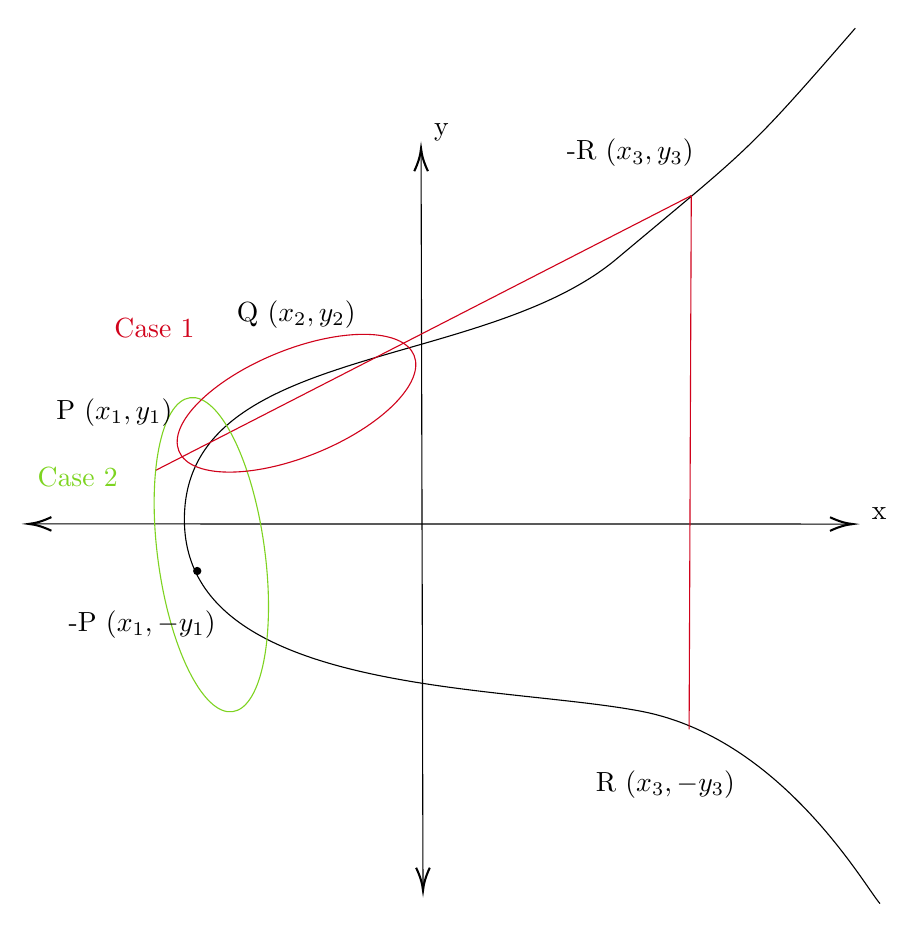
\begin{tikzpicture}[x=0.75pt,y=0.75pt,yscale=-1,xscale=1]
%uncomment if require: \path (0,483); %set diagram left start at 0, and has height of 483

%Straight Lines [id:da532177365763133] 
\draw    (105,268.22) -- (498,268.29) ;
\draw [shift={(500,268.29)}, rotate = 180.01] [color={rgb, 255:red, 0; green, 0; blue, 0 }  ][line width=0.75]    (10.93,-3.29) .. controls (6.95,-1.4) and (3.31,-0.3) .. (0,0) .. controls (3.31,0.3) and (6.95,1.4) .. (10.93,3.29)   ;
\draw [shift={(103,268.22)}, rotate = 0.01] [color={rgb, 255:red, 0; green, 0; blue, 0 }  ][line width=0.75]    (10.93,-3.29) .. controls (6.95,-1.4) and (3.31,-0.3) .. (0,0) .. controls (3.31,0.3) and (6.95,1.4) .. (10.93,3.29)   ;
%Straight Lines [id:da20953626690843463] 
\draw    (292.03,89.34) -- (292.96,442.8) ;
\draw [shift={(292.97,444.8)}, rotate = 269.85] [color={rgb, 255:red, 0; green, 0; blue, 0 }  ][line width=0.75]    (10.93,-3.29) .. controls (6.95,-1.4) and (3.31,-0.3) .. (0,0) .. controls (3.31,0.3) and (6.95,1.4) .. (10.93,3.29)   ;
\draw [shift={(292.02,87.34)}, rotate = 89.85] [color={rgb, 255:red, 0; green, 0; blue, 0 }  ][line width=0.75]    (10.93,-3.29) .. controls (6.95,-1.4) and (3.31,-0.3) .. (0,0) .. controls (3.31,0.3) and (6.95,1.4) .. (10.93,3.29)   ;
%Curve Lines [id:da5778038832019325] 
\draw    (513.17,451.17) .. controls (506.17,443.54) and (466.18,371.6) .. (398.18,358.51) .. controls (330.18,345.42) and (177.98,351.06) .. (178,266.05) .. controls (178.01,181.04) and (321.21,195.02) .. (386.22,140.54) .. controls (451.22,86.06) and (448.22,90.42) .. (501.23,29.4) ;
%Straight Lines [id:da5088539639588137] 
\draw [color={rgb, 255:red, 208; green, 2; blue, 27 }  ,draw opacity=1 ]   (164.2,242.4) -- (422.22,110.03) ;
%Straight Lines [id:da3019672495535983] 
\draw [color={rgb, 255:red, 208; green, 2; blue, 27 }  ,draw opacity=1 ]   (422.22,110.03) -- (421.18,367.23) ;
%Shape: Free Drawing [id:dp6112864843116634] 
\draw  [line width=3] [line join = round][line cap = round] (184.19,290.9) .. controls (184.19,290.9) and (184.19,290.9) .. (184.19,290.9) ;
%Shape: Ellipse [id:dp9247315052804184] 
\draw  [color={rgb, 255:red, 126; green, 211; blue, 33 }  ,draw opacity=1 ] (201.23,358.68) .. controls (187.11,360.59) and (171.08,328.28) .. (165.42,286.51) .. controls (159.75,244.74) and (166.61,209.33) .. (180.73,207.41) .. controls (194.84,205.5) and (210.88,237.81) .. (216.54,279.58) .. controls (222.2,321.35) and (215.35,356.77) .. (201.23,358.68) -- cycle ;
%Shape: Ellipse [id:dp6062445859961849] 
\draw  [color={rgb, 255:red, 208; green, 2; blue, 27 }  ,draw opacity=1 ] (175.36,233.11) .. controls (169.99,219.91) and (191.01,198.9) .. (222.3,186.17) .. controls (253.59,173.45) and (283.31,173.83) .. (288.67,187.03) .. controls (294.04,200.22) and (273.02,221.24) .. (241.73,233.96) .. controls (210.44,246.69) and (180.72,246.31) .. (175.36,233.11) -- cycle ;

% Text Node
\draw (508,259.25) node [anchor=north west][inner sep=0.75pt]  [rotate=-0.01] [align=left] {x};
% Text Node
\draw (297.03,73.94) node [anchor=north west][inner sep=0.75pt]  [rotate=-0.01] [align=left] {y};
% Text Node
\draw (115.01,206.57) node [anchor=north west][inner sep=0.75pt]  [rotate=-0.01] [align=left] {P ($x_1, y_1$)};
% Text Node
\draw (361.03,81.58) node [anchor=north west][inner sep=0.75pt]  [rotate=-0.01] [align=left] {\mbox{-}R ($x_3, y_3$)};
% Text Node
\draw (374.98,385.64) node [anchor=north west][inner sep=0.75pt]  [rotate=-0.01] [align=left] {R ($x_3, -y_3$)};
% Text Node
\draw (202.01,159.57) node [anchor=north west][inner sep=0.75pt]  [rotate=-0.01] [align=left] {Q ($x_2, y_2$)};
% Text Node
\draw (121.01,308.57) node [anchor=north west][inner sep=0.75pt]  [rotate=-0.01] [align=left] {\mbox{-}P ($x_1, -y_1$)};
% Text Node
\draw (143,168) node [anchor=north west][inner sep=0.75pt]   [align=left] {\textcolor[rgb]{0.82,0.01,0.11}{Case 1}};
% Text Node
\draw (106,240) node [anchor=north west][inner sep=0.75pt]   [align=left] {\textcolor[rgb]{0.49,0.83,0.13}{Case 2}};


\end{tikzpicture}
\end{center}


\subsection{Elliptic Curve Operations}

\subsubsection{Case-1: Points \(P\) and \(Q\) on a Line}

Consider the equation of a line:
\[ y = mx + c \quad \text{(Eqn (a))} \]

where \( m = \frac{y_2 - y_1}{x_2 - x_1} \) and \( c = y_1 - mx_1 = y_2 - mx_2 \). All points on this line satisfy Eqn (a).

This line intersects the curve at some point. Substituting \( y = mx + c \) into the curve equation yields:
\[ y^2 = x^3 + ax + b \]
\[ (mx + c)^2 = x^3 + ax + b \]
\[ m^2x^2 + 2mxc + c^2 = x^3 + ax + b \]
\[ x^3 - m^2x^2 + (a - 2mc)x + (b - c^2) = 0 \]

Since \( (x_1, y_1) \) and \( (x_2, y_2) \) satisfy this equation, another solution \( (x_3, y_3) \) can be obtained:
\[ x_1 + x_2 + x_3 = m^2 \]
\[ x_3 = m^2 - x_1 - x_2 \]

And:
\[ y_3 = y_1 + m(x_3 - x_1) \]

So, \( R(x_3, y_3) = P + Q \).\\

\textbf{\underline{Case-2:}}\\
P = $(x_1,y_1)$\\
Q = $(x_2,y_2)$\\
where $x_1=x_2, y_1=-y_2$\\
In this case\\
\begin{center}
    $P \ \boxed{+} Q\ =\ \theta$
\end{center}
\textbf{\underline{Case-3:}}\\
P = $(x_1,y_1)$\\
Q = $(x_2,y_2)$\\
where $x_1=x_2, y_1=y_2$\\
\begin{center}
    $y = mx+c$\\
    $y_2=x_3+ax+b$\\
    $\implies$ $2y\frac{dy}{dx}\ =\ 3x^2+a$\\
    $\implies$ $\frac{dy}{dx}\ =\ \frac{3x^2+a}{2y}$\\
    ${(\frac{dy}{dx})}_{(x_1,y_1)}$ = $\frac{3{x_1}^2+a}{2y_1}$ = m\\
    \vspace{3mm}
    c = $y_1-mx_1$\\
\end{center}
Let us substitute in curve
\begin{center}
    $y_2=x_3+ax+b$\\
    $\implies$${(mx+c)}^2 = x_3+ax+b$\\
    $x_1+x_2+x_3=m^2$\\
    $\implies$$x_3=m^2-x_1-x_2$\\
    $m = \frac{y_3-y_1}{x_3-x_1}$\\
    $\implies$ $y_3 = y_1+m(x_3-x_1)$\\
    R$\rightarrow(x_3,-y_3)$\\
\end{center}
Now, we will be considering the same curve in $\mathbb{Z_P}\ \times\ \mathbb{Z_P}$, where P is a prime number.
\begin{center}
    $y^2=x^3+ax+b$, where (x,y)$\in$ $\mathbb{Z_P}\ \times\ \mathbb{Z_P}$ and a, b $\in\ \mathbb{Z_P}$\\
    $4a^3+27b^2\ \neq\ 0\ mod\ P$\\
\end{center}
Since, we are now working on discrete values, we will not obtain this curve. We will obtain points.\\
\\
\subsection{Case-1: Points \(P\) and \(Q\) on a Line}

For \(P(x_1, y_1)\) and \(Q(x_2, y_2)\), where \(x_2 \neq x_1\), the slope \(m\) between \(P\) and \(Q\) is given by:
\[ m = \frac{y_2 - y_1}{x_2 - x_1} \]

Now, to obtain the \(x\)-coordinate of the third point \(x_3\), we take the inverse of \(x_2 - x_1\) modulo \(P\). Since \(x_2\) and \(x_1\) are distinct, \(x_2 - x_1\) will be non-zero, and its inverse modulo \(P\) exists because \(P\) is prime:
\[ m = (y_2 - y_1) \times (x_2 - x_1)^{-1} \mod P \]

Thus, the \(y\)-coordinate \(y_3\) of the third point \(R\) is given by:
\[ y_3 = y_1 + m(x_3 - x_1) \in ZP \]

\subsection{Elliptic Curve in Discrete Domain}

Now consider the curve in the discrete domain \( ZP \times ZP \), where \( P \) is a prime number:

\[ y^2 = x^3 + ax + b \]

with \( (x,y) \in ZP \times ZP \) and \( a, b \in ZP \). Ensure that \( 4a^3 + 27b^2 \neq 0 \) mod \( P \). In this discrete context, points are obtained instead of the curve itself.

\section{Elliptic Curve Diffie-Hellman (ECDH)}

Consider the scenario where Alice and Bob want to exchange messages securely. They both have access to a public curve \(E\) and a base point \(P\), denoted as \((E, P)\), which is publicly known.

\subsection{Key Generation}

\textbf{Alice:}
\begin{itemize}
    \item \textbf{Secret Key:} \(a\)
    \item \textbf{Public Key:} \(aP\)
\end{itemize}

\textbf{Bob:}
\begin{itemize}
    \item \textbf{Secret Key:} \(b\)
    \item \textbf{Public Key:} \(bP\)
\end{itemize}


\tikzset{every picture/.style={line width=0.75pt}} %set default line width to 0.75pt        

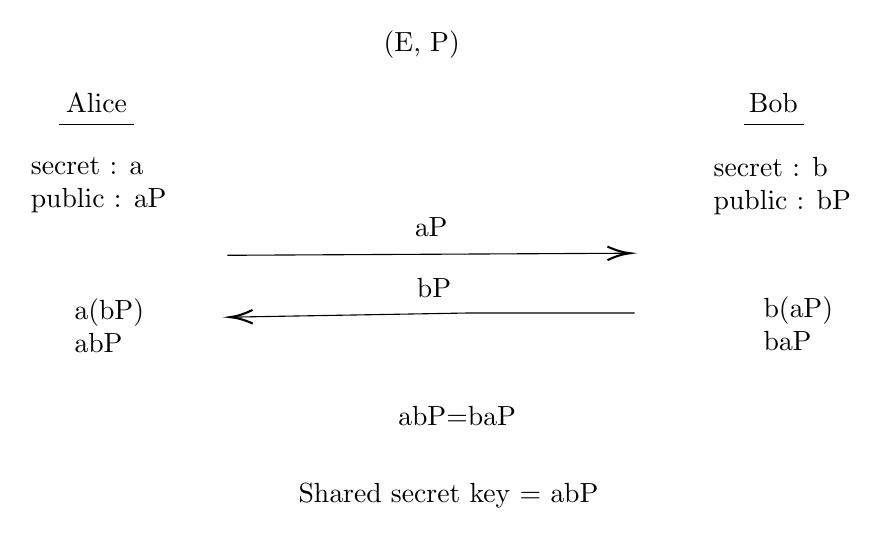
\begin{tikzpicture}[x=0.75pt,y=0.75pt,yscale=-1,xscale=1]
%uncomment if require: \path (0,300); %set diagram left start at 0, and has height of 300

%Straight Lines [id:da1435011466169438] 
\draw    (137,64.4) -- (173,64.4) ;
%Straight Lines [id:da7210376025319416] 
\draw    (467,64.4) -- (496,64.4) ;
%Straight Lines [id:da03246958013588985] 
\draw    (218,127.4) -- (319.21,126.88) -- (410,126.41) ;
\draw [shift={(412,126.4)}, rotate = 179.7] [color={rgb, 255:red, 0; green, 0; blue, 0 }  ][line width=0.75]    (10.93,-3.29) .. controls (6.95,-1.4) and (3.31,-0.3) .. (0,0) .. controls (3.31,0.3) and (6.95,1.4) .. (10.93,3.29)   ;
%Straight Lines [id:da47817176973288045] 
\draw    (414.2,155.2) -- (334.2,155.2) -- (221.2,157.17) ;
\draw [shift={(219.2,157.2)}, rotate = 359] [color={rgb, 255:red, 0; green, 0; blue, 0 }  ][line width=0.75]    (10.93,-3.29) .. controls (6.95,-1.4) and (3.31,-0.3) .. (0,0) .. controls (3.31,0.3) and (6.95,1.4) .. (10.93,3.29)   ;

% Text Node
\draw (139,48) node [anchor=north west][inner sep=0.75pt]   [align=left] {Alice};
% Text Node
\draw (468,48) node [anchor=north west][inner sep=0.75pt]   [align=left] {Bob};
% Text Node
\draw (122,79) node [anchor=north west][inner sep=0.75pt]   [align=left] {secret : a\\public : aP};
% Text Node
\draw (292,18) node [anchor=north west][inner sep=0.75pt]   [align=left] {(E, P)};
% Text Node
\draw (451,79) node [anchor=north west][inner sep=0.75pt]   [align=left] {secret : b\\public : bP};
% Text Node
\draw (307,108) node [anchor=north west][inner sep=0.75pt]   [align=left] {aP};
% Text Node
\draw (308,137) node [anchor=north west][inner sep=0.75pt]   [align=left] {bP};
% Text Node
\draw (143,147) node [anchor=north west][inner sep=0.75pt]   [align=left] {a(bP)\\abP};
% Text Node
\draw (475,146) node [anchor=north west][inner sep=0.75pt]   [align=left] {b(aP)\\baP};
% Text Node
\draw (299,199) node [anchor=north west][inner sep=0.75pt]   [align=left] {abP=baP};
% Text Node
\draw (251,236) node [anchor=north west][inner sep=0.75pt]   [align=left] {Shared secret key = abP};


\end{tikzpicture}
\end{center}

\subsection{Key Exchange}

To generate a shared secret key, Alice and Bob perform the following computations:
\begin{align*}
    \text{Alice:} & \quad a(bP) = abP \\
    \text{Bob:} & \quad b(aP) = baP
\end{align*}

Since the operation is commutative in elliptic curve arithmetic, \(abP = baP\). Thus, both Alice and Bob end up with the same shared secret key \(abP = baP\).

\subsection{Security Considerations}

The security of ECDH relies on the computational difficulty of finding \(xP\) from \(P\), known as the Discrete Logarithm Problem on Elliptic Curves.

\textbf{Note:} The elliptic curve calculations can be visualized and executed using tools like Jupyter Notebook, with code available from resources like SageMath.

\section{Elliptic Curve Digital Signature Algorithm (ECDSA)}

In ECDSA, cryptographic operations are performed using elliptic curves. Let \((E, P)\) denote the public keys, where \(E\) represents the elliptic curve and \(P\) is a base point on the curve. Each party, say Alice, possesses a secret key \(d_A\) and a corresponding public key \(Q_A = d_A \cdot P\).

\subsection{Signature Generation}

Given a message \(m\) to be signed, the signer (Alice) computes the signature \(s\) using her secret key \(d_A\):
\[ s = k^{-1} (z + r \cdot d_A) \mod n \]
where \(k\) is a randomly generated number, \(z\) is the hash of the message, \(r\) is the \(x\)-coordinate of the point resulting from \(k \cdot P\) on the curve, and \(n\) is a large prime number associated with the curve.

\subsection{Signature Verification}

The verifier (Bob) receives the message \(m\), along with the signature \(s\) and the public key \(Q_A\). Bob then computes:
\[ r = \text{the } x\text{-coordinate of} \left( (s \cdot Q_A - z \cdot G) \cdot w \right) \]
where \(G\) is the base point, \(w\) is the multiplicative inverse of \(s\) modulo \(n\), and \(z\) is the hash of the message. If \(r\) matches the \(x\)-coordinate of the original signature, the signature is considered authentic.

ECDSA ensures message integrity and authenticity in cryptographic communications, offering a robust mechanism for digital signature generation and verification.


\tikzset{every picture/.style={line width=0.75pt}} %set default line width to 0.75pt        

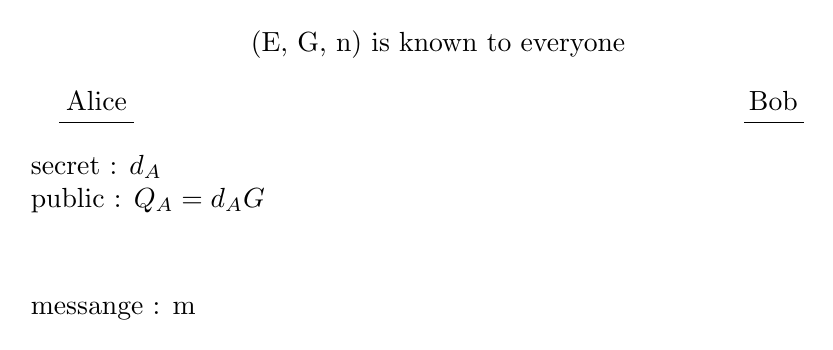
\begin{tikzpicture}[x=0.75pt,y=0.75pt,yscale=-1,xscale=1]
%uncomment if require: \path (0,300); %set diagram left start at 0, and has height of 300

%Straight Lines [id:da1435011466169438] 
\draw    (137,64.4) -- (173,64.4) ;
%Straight Lines [id:da7210376025319416] 
\draw    (467,64.4) -- (496,64.4) ;

% Text Node
\draw (139,48) node [anchor=north west][inner sep=0.75pt]   [align=left] {Alice};
% Text Node
\draw (468,48) node [anchor=north west][inner sep=0.75pt]   [align=left] {Bob};
% Text Node
\draw (122,79) node [anchor=north west][inner sep=0.75pt]   [align=left] {secret : $d_A$\\public : $Q_A = d_AG$};
% Text Node
\draw (228,19) node [anchor=north west][inner sep=0.75pt]   [align=left] {(E, G, n) is known to everyone};
% Text Node
\draw (122,150) node [anchor=north west][inner sep=0.75pt]   [align=left] {messange : m};


\end{tikzpicture}
\end{center}



\subsection{Signature Generation}
1. \textbf{Hash Calculation:} Compute the hash of the message \( m \), denoted as \( e \). \\
2. \textbf{Bit Extraction:} Extract \( L_n \) leftmost bits of \( e \), where \( L_n \) is the bit length of \( n \). \\
3. \textbf{Random Number Generation:} Generate a random number \( K \) from the range \([1, n-1]\). \\
4. \textbf{Point Computation:} Compute the point \((x_1, y_1) = K \cdot G\), where \( G \) is the base point on the curve. \\
5. \textbf{Signature Components:}
   - Calculate \( r = x_1 \mod n \). If \( r = 0 \), return to step 3.
   - Compute \( s = K^{-1} \cdot [Z + r \cdot d_A] \mod n \), where \( d_A \) is the signer's secret key.
   - If \( s = 0 \), return to step 3.
6. \textbf{Signature Generation:} Generate the signature \((r, s)\) for the message \( m \).

\subsection{Signature Verification (by Bob)}
1. \textbf{Validity Checks:}
   - Verify that \( Q_A \neq 0 \).
   - Check if \( Q_A \) lies on the curve \( E \).
   - Ensure that \( n \cdot Q_A = d_A \cdot (n \cdot G) = 0 \).
2. \textbf{Verification Steps:}
   - Verify that \( r \) and \( s \) are within the range \([1, n-1]\).
   - Compute \( e = \text{Hash}(m) \).
   - Extract \( L_n \) leftmost bits of \( e \) to obtain \( Z^- \).
   - Calculate \( u_1 = Z^- \cdot s^{-1} \mod n \) and \( u_2 = r \cdot s^{-1} \mod n \).
   - Perform point addition: \((x_2, y_2) = u_1 \cdot G + u_2 \cdot Q_A\).
   - If \((x_2, y_2) = 0\), the signature is invalid.
   - Check if \( r \equiv x_2 \mod n \). If true, the signature is valid; otherwise, it's invalid.

\subsection{Proof of Validity}
The verification involves computing \( c = u_1 \cdot G + u_2 \cdot Q_A \), where \( c \) is the computed point. By substituting the value of \( s^{-1} \), it can be shown that \( c = K \cdot G \), thus proving the validity of the signature.

\end{document}